\section{Visión artificial}

\begin{frame}\frametitle{¿Qué es la visión computacional?}
  \begin{itemize}
  \item \textbf{Visión Humana: } Se puede concebir como una tarea de procesamiento de información, que obtiene significado a partir de los estímulos percibidos por los ojos.
  \item \textbf{Visión Computacional: } Desarrollo de programas de computadora que puedan \textit{interpretar} imágenes. Es decir, realizar la visión humana por medios computacionales. 
  \end{itemize}
  \begin{figure}
    \centering
    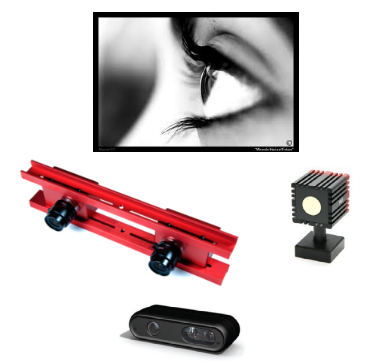
\includegraphics[width=0.5\textwidth]{Figures/ComputerVision.png}
  \end{figure}
\end{frame}

\begin{frame}\frametitle{Teoría de Marr}
“Visión es un proceso que produce, a partir de imágenes del mundo externo, una descripción que es útil para el observador y que está libre de información irrelevante.” (Marr, 1976).\\
El fenómeno de la visión lo podemos considerar como el producto de un sistema de procesamiento de información.\\

Marr propone los siguientes tres niveles de construcción de un sistema de procesamiento de información:\\
\begin{enumerate}
\item Teoría Computacional (¿Cuál es el problema por resolver?)
\item Representación y algoritmos (Estrategía usada para resolverlo)
\item Implementación (Realización física, software y hardware)
\end{enumerate}
Es decir, la visión computacional sería un proceso parecido a la visión humana, similar en los niveles computacionales y de algoritmos, pero implementado de forma diferente: en hardware de procesamiento con sensores de visión. 
\end{frame}

\begin{frame}\frametitle{Visión Computacional}
  Por lo tanto, la tarea de la Visión por computadora es la construcción de descriptores de la escena con base en características relevantes contenidas en una imagen:
  \begin{columns}
    \begin{column}{0.5\textwidth}
\begin{figure}
    \centering
    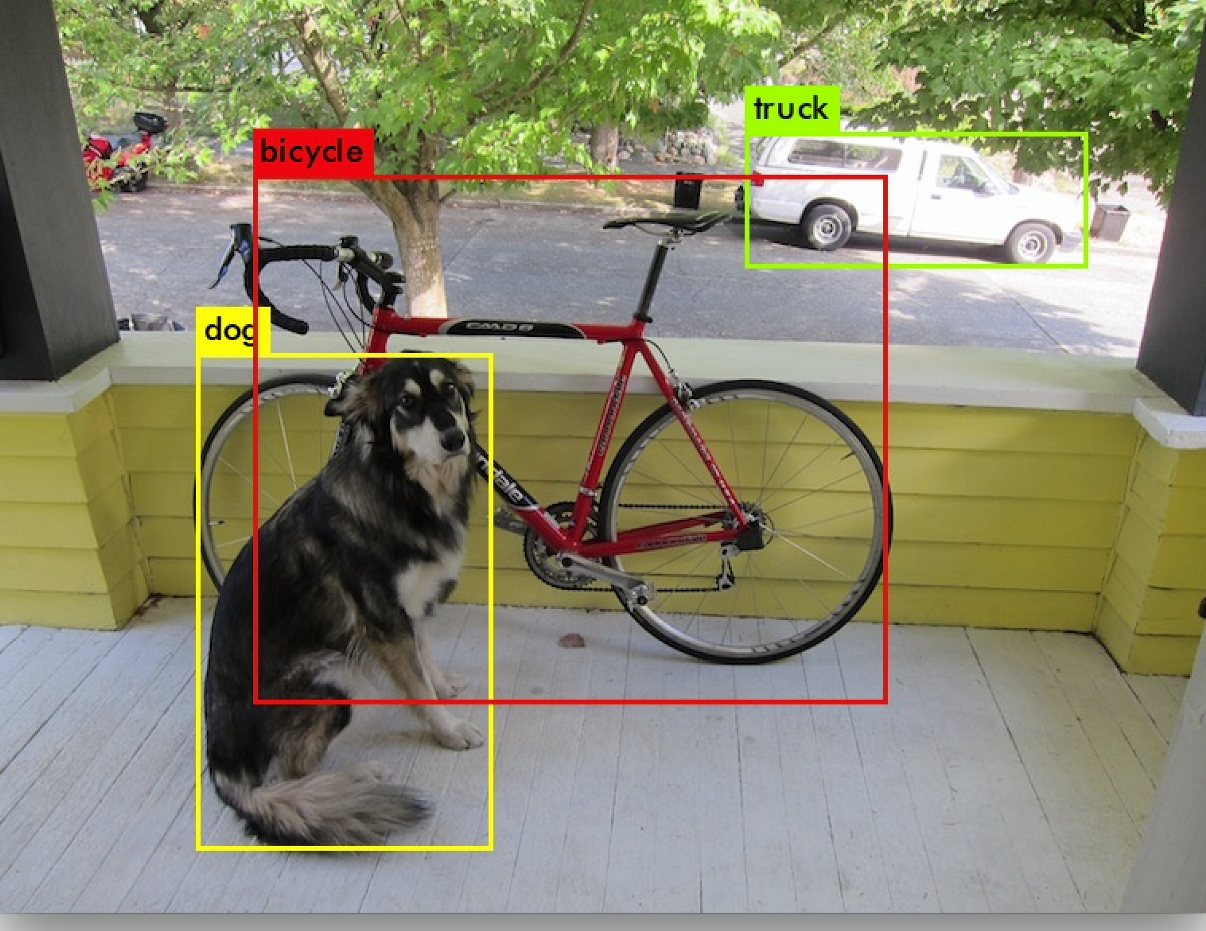
\includegraphics[width=0.8\textwidth]{Figures/YoloExample.png}
\end{figure}
    \end{column}
    \begin{column}{0.5\textwidth}
\begin{itemize}
\item Objetos
\item Formas de Superficies
\item Colores
\item Texturas
\item Movimientos
\item Iluminación
\item Reflejos
\end{itemize}
    \end{column}
    \end{columns}
\end{frame}

\begin{frame}\frametitle{Vision Computacional vs Proc de Imágenes}
\begin{enumerate}
\item Procesamiento de imagenes: Es cualquier forma de procesamiento de señales donde la entrada es una imagen, la salida puede ser otra imagen o un conjunto de características o parámetros relacionados con la misma.
\item Visión Computacional: Estudio y aplicación de métodos que permiten a las computadoras “entender” el contenido de una imagen.
\item Visión Máquina: Es la aplicación de la visión por computadora en la industria y procesos de manufactura.
\end{enumerate}

\end{frame}

\begin{frame}\frametitle{Aplicaciones}
  Tareas que se pueden hacer con visión computacional (con aplicaciones a la robótica):
  \begin{itemize}
  \item OCR (Optical Character Recognition)
  \item Detección e identificación de rostros
  \item Reconocimiento de objetos
  \item Percepción para vehículos sin conductor
  \item Reconocimiento de gestos
  \end{itemize}
  Otras aplicaciones:
  \begin{itemize}
  \item Vigilancia
  \item Imagenología médica
  \item Consultas a bases de datos de imágenes.
  \item Percepción remota
  \end{itemize}
\end{frame}


\begin{frame}\frametitle{Esquema de Visión}
  \begin{figure}
    \centering
    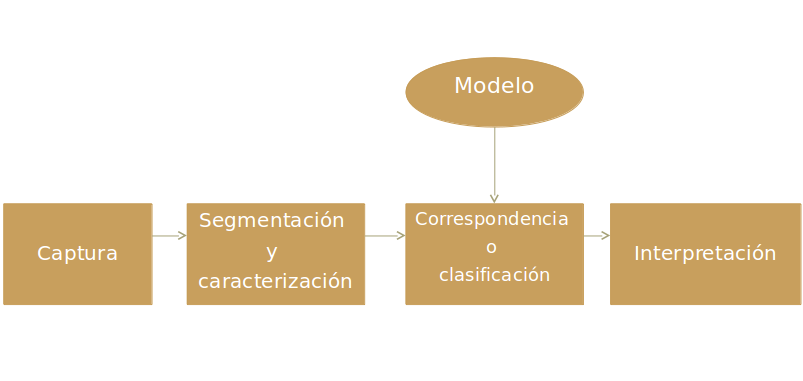
\includegraphics[width=1.0\textwidth]{Figures/VisionGeneralProcess.png}
  \end{figure}
\end{frame}


\begin{frame}\frametitle{Dificultades}

  El entorno real tiene una gran cantidad de variaciones en las imágenes de entrada.
  \begin{columns}
    \begin{column}{0.5\textwidth}
\begin{figure} %this figure will be at the right
    \centering
    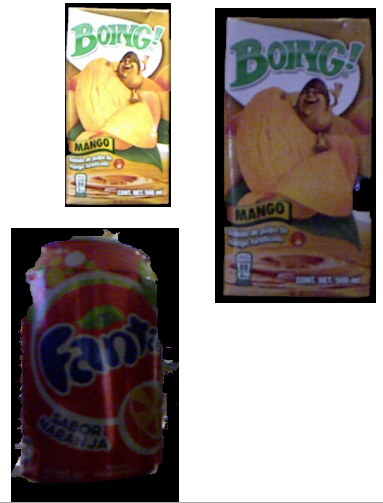
\includegraphics[width=0.5\textwidth]{Figures/ComputerVisionProblems.png}
\end{figure}
    \end{column}
    \begin{column}{0.5\textwidth}
\begin{enumerate}
\item Iluminación
\item Orientación
\item Oclusión
\item Escala
\item Ruido
\item Desenfoque
\end{enumerate}
    \end{column}
  \end{columns}
\end{frame}

\begin{frame}\frametitle{Hardware y Software}
La computación con imágenes tiene mas de 30 años, sin embargo, en los últimos años, se ha incrementado considerablemente su desarrollo debido a:
\begin{enumerate}
\item Decremento en los precios 
\item Memoria con gran capacidad
\item Procesadores de propósito general de alta velocidad.
\item Existen scanners o camaras digitales que pueden ser utilizados para procesar imágenes propias.
\item Existen bibliotecas de software que contienen subrutinas de procesamiento de imágenes (opencv).
\end{enumerate}
\end{frame}

\begin{frame}\frametitle{OpenCV}
  \begin{columns}
    \begin{column}{0.5\textwidth}
      \begin{figure}
        \centering
        
\includegraphics[width=0.6\textwidth]{Figures/OpenCVLogo.png}
      \end{figure}
    \end{column}
    \begin{column}{0.5\textwidth}
      OpenCV es una biblioteca libre de visión artificial, originalmente desarrollada por Intel.
      
      Programación en código  Python, C y C++
      
      Existen versiones para GNU/Linux, Mac OS X y Windows
    \end{column}
    \end{columns}
    \end{frame}

\begin{frame}\frametitle{OpenCV}
\begin{figure}[h!]
        \centering
        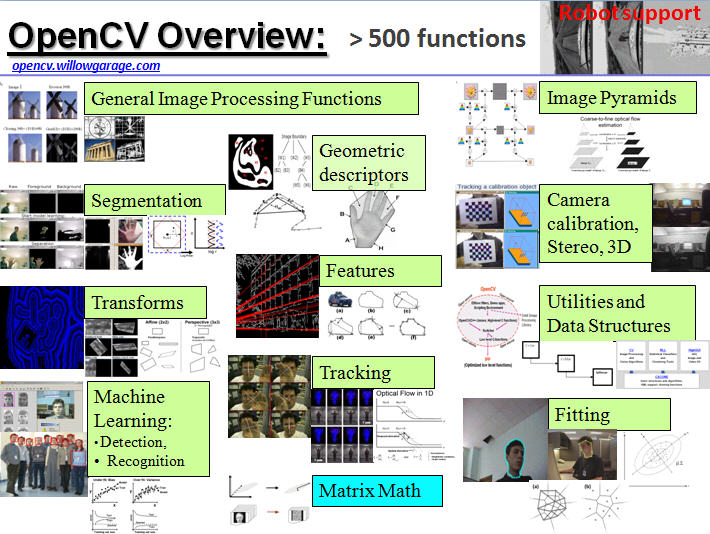
\includegraphics[width=0.75\textwidth]{Figures/OpenCVOverview.png}
\end{figure}
\end{frame}


\begin{frame}\frametitle{Imágenes como funciones}
  \begin{itemize}
  \item Una imagen (en escala de grises) es una función $I(x,y)$ donde $x,y$ son variables discretas en coordenadas de imagen y la función $I$ es intensidad luminosa.
    \item Las imágenes también pueden considerarse como arreglos bidimensionales de números entre un mínimo y un máximo (usualmente 0-255).
    \item Las imágenes de color son funciones vectoriales $f:\mathbb{R}^2\rightarrow \mathbb{R}^3$ donde cada componente de la función se llama canal.
%  \[I(x,y) = \left[\begin{tabular}{c}$r(x,y)$\\$g(x,y)$\\$b(x,y)$\end{tabular}\right]\]
  \end{itemize}
  \begin{figure}
    \centering
    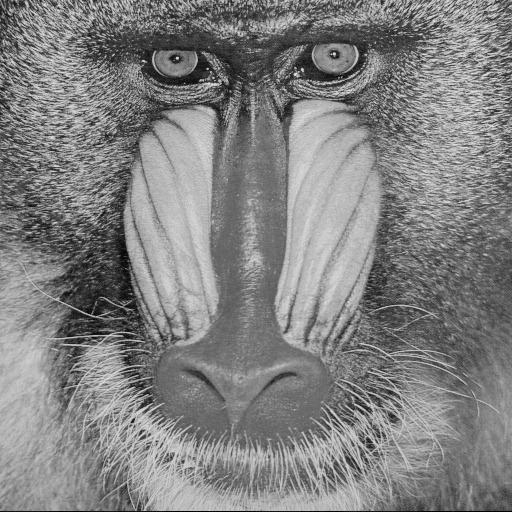
\includegraphics[width=0.3\textwidth]{Figures/baboon_grayscale.jpg}
    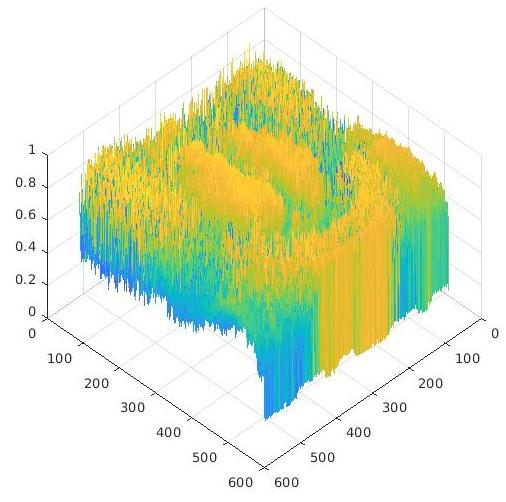
\includegraphics[width=0.35\textwidth]{Figures/BaboonPlot.jpg}
  \end{figure}
\end{frame}

\begin{frame}\frametitle{Las imágenes como funciones}
    Aunque formalmente una imagen es un mapeo $f:\mathbb{R}^2\rightarrow \mathbb{R}$, en la práctica, tanto $x,y$ como $I$ son varialbes discretas con valores entre un mínimo y un máximo.
\begin{figure}
  \centering
  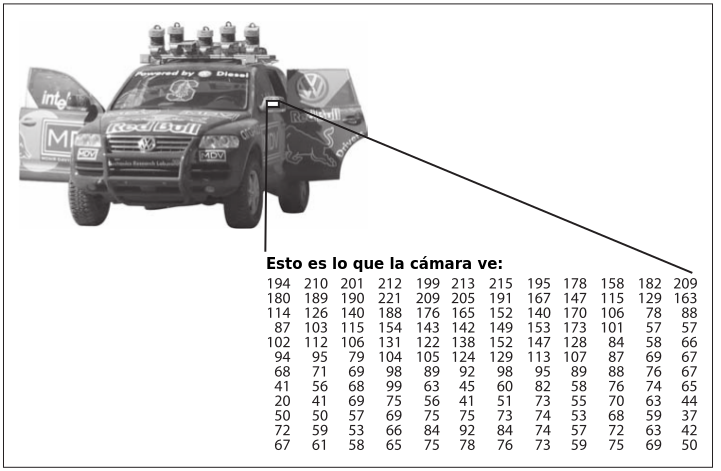
\includegraphics[width=0.45\textwidth]{Figures/ImageRepresentation.png}
\end{figure}
\end{frame}


\begin{frame}\frametitle{Operaciones básicas}
  \begin{itemize}
  \item Desfase
  \item Escalamiento
  \item Inversión en $x,y$
  \item Suma y Resta 
  \item Multiplicación
  \end{itemize}
\end{frame}

\begin{frame}\frametitle{Tipos de ruido}
  El ruido es una señal aleatoria $\eta(x,y)$, es decir, no sabemos cuánto vale para un punto determinado $(x,y)$ pero sí podemos caracterizarla.
  \[I_n(x,y) = I(x,y) + \eta(x,y)\]
  Existen varios tipos de ruido:
  \begin{itemize}
  \item Sal y pimienta: aleatoriamente aparecen puntos ya sea blancos o negros
  \item Ruido de impulso: aleatoriamente aparecen puntos blancos
  \item Ruido gausiano: $\eta(x,y)$ se distribuye normalmente
  \end{itemize}
\end{frame}

% \begin{frame}\frametitle{Tarea 11 - Herramientas de visión artificial}
% \end{frame}

\begin{frame}\frametitle{Espacios de color}
  Un espacio de color o modelo de color es una representación del color mediante un conjunto numérico de valores, generalmente tres valores. Existen varios espacios de color:
  \begin{columns}
    \begin{column}{0.5\textwidth}
      \begin{itemize}
      \item Aditivos:
        \begin{itemize}
        \item RGB
        \item HSV
        \item YCrCb
        \end{itemize}
      \item Sustractivos
        \begin{itemize}
        \item MCYK
        \end{itemize}
      \end{itemize}
    \end{column}
    \begin{column}{0.5\textwidth}
      \begin{itemize}
      \item Lineales:
        \begin{itemize}
        \item RGB
        \item CIE XYZ
        \end{itemize}
      \item No lineales
        \begin{itemize}
        \item HSV
        \item HSI 
        \end{itemize}
      \end{itemize}
    \end{column}
  \end{columns}
\end{frame}

\begin{frame}\frametitle{El espacio RGB}
  En este espacio cada color se forma mediante la suma de tres colores primarios: rojo, verde y azul. 
  \begin{figure}
    \centering
    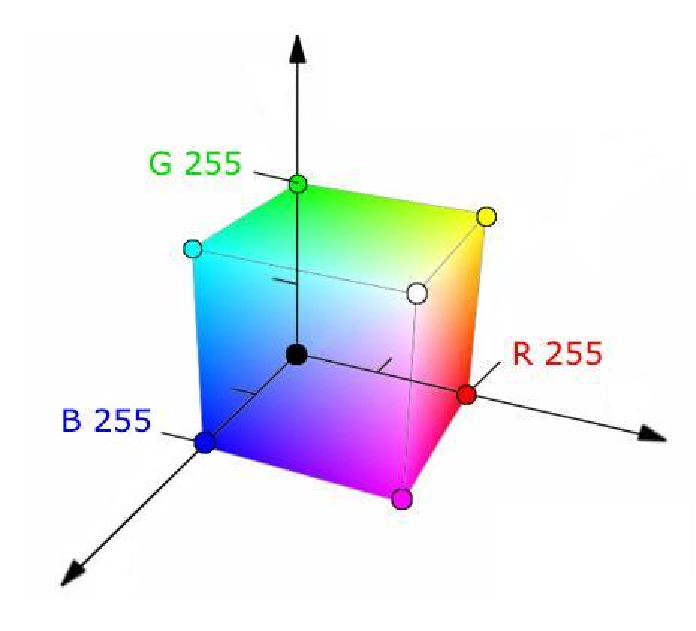
\includegraphics[width=0.33\textwidth]{Figures/RGB_model.pdf}
    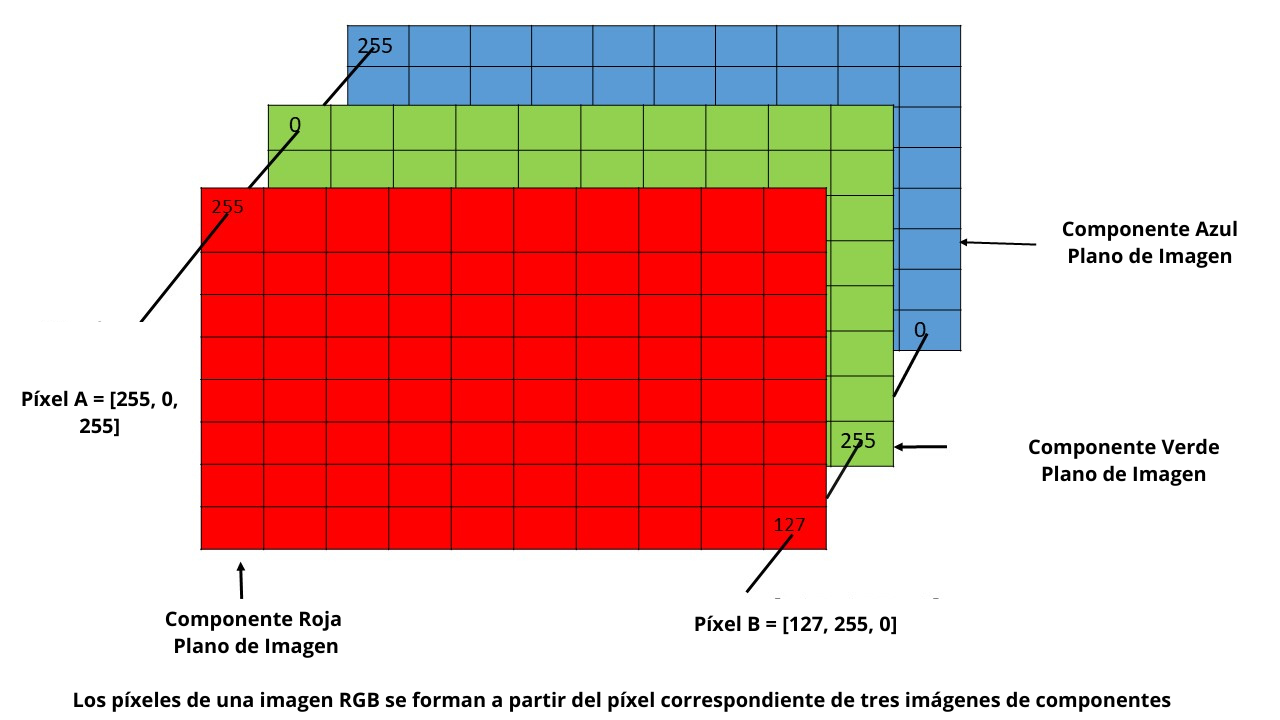
\includegraphics[width=0.5\textwidth]{Figures/rgb_pixels.png}
  \end{figure}
  En memoria, las imágenes RGB se suelen representar con arreglos de $H\times W \times 3$ donde $H$ y $W$ son el alto y ancho de la imagen respectivamente. 
\end{frame}

\begin{frame}\frametitle{El espacio HSV}
  Es un espacio de color diseñado para representar el color de una forma más similar a como lo percibe el ojo humano. El color se representa con tres valores:
  \begin{itemize}
  \item \textbf{Hue:} (Matiz) Es el atributo del color que hace que un estímulo se perciba como similar a alguno de los colores que el ojo puede percibir: rojo, amarillo, verde, azul, violeta, o una combinación de ellos.
  \item \textbf{Saturaion: } (Saturación) Es el atributo que indica qué tan colorido es un estímulo con respecto a su propio brillo.
  \item \textbf{Value: } (Valor) Atributo que indica qué tanta luz emite un estímulo. 
  \end{itemize}
  \begin{columns}
    \begin{column}{0.35\textwidth}
      \begin{figure}
        \centering
        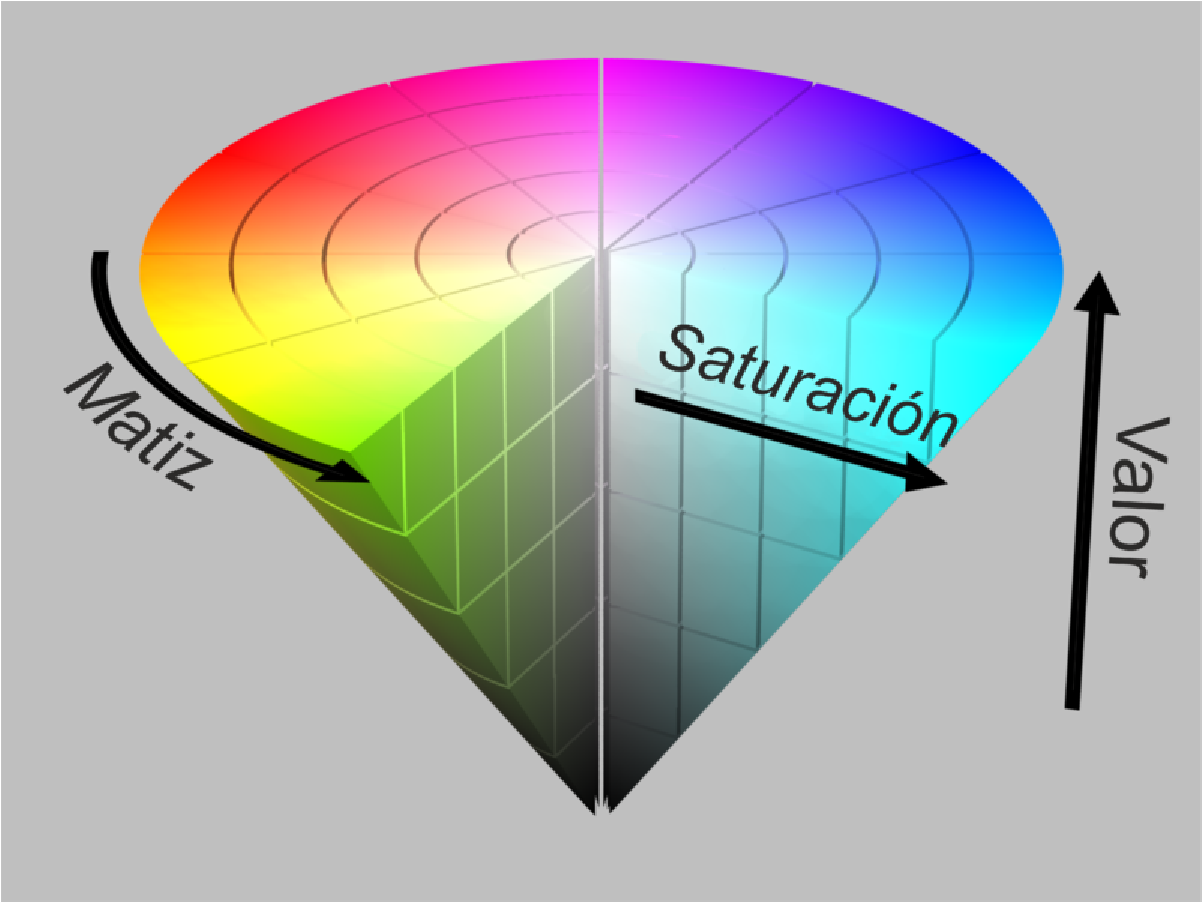
\includegraphics[width=\textwidth]{Figures/hsv_space.pdf}
      \end{figure}
    \end{column}
    \begin{column}{0.65\textwidth}
      Para obtenerlo a partir de RGB:
      \[M = \max(R,G,B)\qquad m=\min(R,G,B)\qquad C=M - m\]
      \[H = \begin{cases}\begin{tabular}{lcl}Indeterminado & si & C=0 \\ $\frac{G-B}{C}\times 60$ & si & M = R \\ $\frac{B - R}{C}\times 60$ & si & M = G \\ $\frac{R - G}{C}\times 60$ & si & M = B\end{tabular}\end{cases}\qquad V = M\]
      \[S = \begin{cases}0\qquad \textrm{si}\; V=0\\ \frac{C}{V}\qquad \textrm{en otro caso}\end{cases}\]
    \end{column}
  \end{columns}
\end{frame}

\begin{frame}\frametitle{Nubes de puntos}
  Las nubes de puntos son conjuntos de vectores que representan puntos en el espacio. Estos vectores generalmente tienen información de posición $(x,y,z)$. También pueden contener información de color $(x,y,z,r,g,b)$.
  \begin{figure}
      \centering
      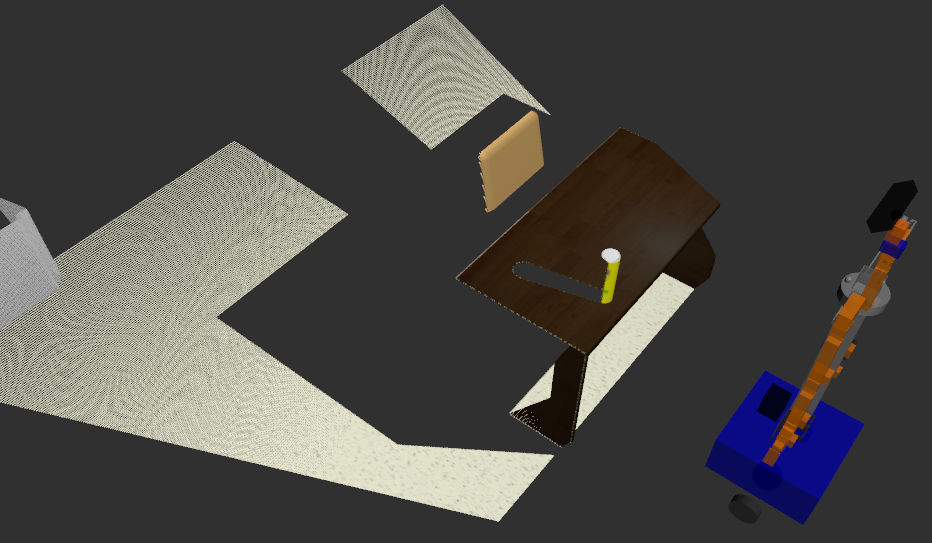
\includegraphics[width=0.5\textwidth]{Figures/CloudExample.png}
  \end{figure}
  Son útiles para determinar la posición en el espacio de los objetos reconocidos. 
\end{frame}

\begin{frame}\frametitle{Segmentación por color}
  La segmentación de una imagen se refiere a obtener regiones significativas con ciertas características. En este caso, la característica es que estén en un cierto intervalo de color. Los pasos generales para esto son:
  \begin{enumerate}
  \item Transformación de la imagen del espacio BGR al HSV (función \texttt{cvtColor})
  \item Obtención de aquellos pixeles que están en un rango de color (función \texttt{inRange})
  \item Eliminación de \textit{outliers}, generalmente con operadores morfológicos (funciones \texttt{erode} y \texttt{dilate})
  \item Obtención del centroide de la región (funciones \texttt{findNonZero} y \texttt{mean})
  \item Si se dispone de una nube de puntos, se puede obtener la posición $(x,y,z)$ del centroide de la región segementada. 
  \end{enumerate}
\end{frame}

\begin{frame}\frametitle{Ejercicio 08 - Segmentación por color}
  \begin{enumerate}
  \item En el archivo \texttt{catkin\_ws/src/students/scripts/assignment08.py}, en la función \texttt{segment\_by\_color}, realice lo siguiente:
    \begin{enumerate}
    \item Defina dos límites superiores y dos límites inferiores, en el espacio de color HSV, para segmentar las latas que se encuentran sobre el escritorio simulado.
    \item Transforme la imagen del espacio BGR al espacio HSV mediante la función \texttt{cvtColor} de OpenCV.
    \item Determine los pixeles de la imagen que pertenecen al rango de color elegido mediante la fucion \texttt{inRange} de OpenCV.
    \item Encuentre los índices de los pixeles que pertenecen al rango de color con la función \texttt{findNonZero} de OpenCV.
    \item Utilizando los índices anteriores y la nube de puntos, determine el centroide del objeto con el color seleccionado. 
    \end{enumerate}
  \item Ejecute la simulación con el comando \texttt{roslaunch bring\_up vision\_examples.launch }
  \item Ejecute la práctica con el comando \texttt{rosrun students assignment08.py}
  \item En la pestaña \textit{Simple Tasks} de la GUI, en el campo \textit{Find Object} teclee \texttt{pringles} o \texttt{drink}
  \item En el visualizador debe dibujarse una esfera morada sobre el centro del objeto seleccionado. 
  \end{enumerate}
\end{frame}

\begin{frame}\frametitle{SLID}
  Un sistema $S$ es un mapeo del conjunto de señales al conjunto de señales, es decir, es algo donde entra una señal $I(x,y)$ y sale otra señal $O(x,y)$:
  \[O(x,y) = S[I(x,y)]\]
  Los sistemas lineales invariantes ante el desfase son sistemas en los que se cumplen las siguientes propiedades:
  \begin{itemize}
  \item \textbf{Aditividad y homogeneidad:}
    \[S[\alpha I_1(x,y) + \beta I_2(x,y)] = \alpha S[I_1(x,y)] + \beta S[I_2(x,y)]\]
  \item \textbf{Invarianza ante el desfase:}
    \[\textrm{Si} \qquad S[I(x,y)] = O(x,y) \qquad\textrm{entonces:}\]
    \[S[I(x-i, y-j)] = O(x-i, y-j) \qquad \forall i,j \in \mathbb{Z}\]
  \end{itemize}
  Los SLID se pueden caracterizar de varias formas:
  \begin{itemize}
  \item Ecuaciones en diferencias
  \item Funciones de transferencia
  \item Respuesta al impulso
  \end{itemize}
\end{frame}

\begin{frame}\frametitle{Convolución}
  Si se conoce la respuesta al impulso $H(x,y)$ de un sistema SLID, se puede obtener la salida $O(x,y)$ ante cualquier entrada $I(x,y)$, mediante la convolución, definida como:
  \[O(x,y) = I(x,y)*H(x,y) = \sum_{i=-\infty}^\infty \sum_{j=-\infty}^\infty I(i,j)H(x-i, y-j)\]
  Ejemplos:
  \[\left[\begin{tabular}{cccc}
      3 & 1 & 4 & 1\\
      5 & 9 & 2 & 6\\
      5 & 3 & 5 & 8\\
      9 & 7 & 9 &3
    \end{tabular}\right]* [1\quad -1] =
  \left[\begin{tabular}{ccccc}
      3 & -2 & 3 & -3 & -1\\
      5 & 4 & -7 & 4 & -6\\
      5 & -2 & 2 & 3 & -8\\
      9 & -2 & 2 & -6 & -3
    \end{tabular}\right]\]

  \[\left[\begin{tabular}{cccc}
      3 & 1 & 4 & 1\\
      5 & 9 & 2 & 6\\
      5 & 3 & 5 & 8\\
      9 & 7 & 9 &3
    \end{tabular}\right]* \left[\begin{tabular}{c}1 \\ -1\end{tabular}\right] =
  \left[\begin{tabular}{cccc}
      3 & 1 & 4 & 1\\
      2 & 8 & -2 & 5\\
      0 & -6 & 3 & 2\\
      4 & 4 & 4 & -5\\
      -9 & -7 & -9 & -3
    \end{tabular}\right]\]
\end{frame}

\begin{frame}\frametitle{Manejo de bordes}
  En el ejemplo anterior, supusimos que fuera de la matriz, todos los elementos son cero. Sin embargo existen otras formas de manejar los borde:
  \begin{itemize}
  \item Recortar: suponer que fuera de la matriz los valores son cero. En el caso de una imagen, suponemos pixeles negros fuera de la imagen.
  \item Wrap around: suponer que la imagen es periódica.
  \item Borde repetido: suponer que los valores de los bordes se mantienen iguales fuera de la imagen.
  \item Reflexión: fuera de los bordes se tiene una imagen en espejo.
  \end{itemize}
\end{frame}

\begin{frame}\frametitle{Propiedades de la convolución}
  \begin{itemize}
  \item Es conmutativa: $H*I = I*H$
  \item Es asociativa: $H*I_1*I_2$ = $H*(I_1*I_2)$ = $(H*I_1)*I_2$
  \item Es distributiva: $H*(I_1 + I_2) = H*I_1 + H*I_2$
  \item Es lineal: $H*(\alpha I_1 + \beta I_2) = \alpha H*I_1 + \beta H*I_2$
  \end{itemize}
  En el caso de secuencias finitas bidimensionales:
  \begin{itemize}
  \item Si $I\in\mathbb{R}^{r_1\times c_1}$ y $H\in\mathbb{R}^{r_2\times c_2}$, entonces $(I*H) \in \mathbb{R}^{(r_1+r_2-1)\times (c_1 + c_2 - 1)}$
  \item Si $I\in\mathbb{R}^{r_1\times c_1}$ y $H\in\mathbb{R}^{r_2\times c_2}$, la complejidad de la convolución es del orden de $r_1 r_2 c_1 c_2$
  \end{itemize}
\end{frame}

\begin{frame}\frametitle{Conexión de sistemas SLID}
  Dos o más SLID se pueden conectar de dos formas distintas:
  \begin{itemize}
  \item Conexión en paralelo:
    \begin{figure}
      \centering
      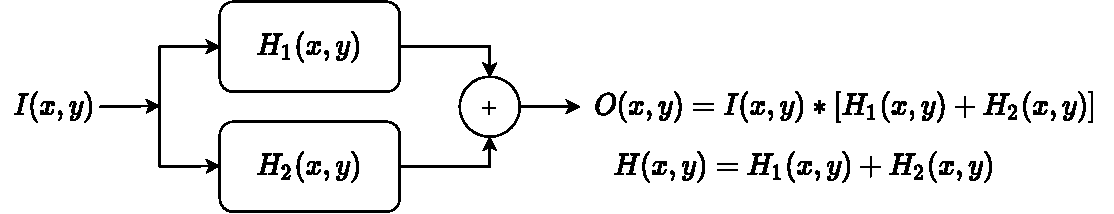
\includegraphics[scale=0.7]{Figures/SLIDParallel.pdf}
    \end{figure}
  \item Conexión en cascada:
    \begin{figure}
      \centering
      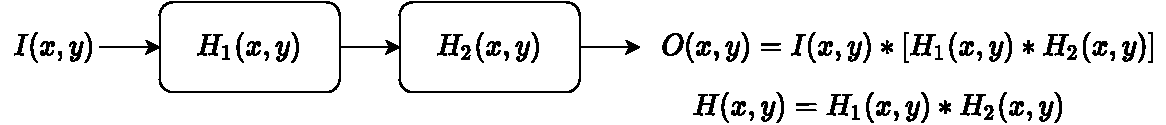
\includegraphics[scale=0.7]{Figures/SLIDCascade.pdf}
    \end{figure}
  \end{itemize}
\end{frame}

\begin{frame}\frametitle{Gradiente}
  El gradiente de una imagen está definido como:
  \[\nabla I = \left[\frac{\partial I}{\partial x}, \frac{\partial I}{\partial y}\right]\]
  Las derivadas parciales se puede aproximar mediante diferencias finitas:
  \begin{eqnarray*}
    \frac{\partial I}{\partial x} &=& \lim_{\Delta x \rightarrow 0}\frac{I(x + \Delta x, y) - I(x,y)}{\Delta x}\approx I_{i,j} - I_{i,j-1}\\
    \frac{\partial I}{\partial y} &=& \lim_{\Delta y \rightarrow 0}\frac{I(x, y + \Delta y) - I(x,y)}{\Delta y}\approx I_{i,j} - I_{i-i,j}
  \end{eqnarray*}
  donde $(i,j)$ representan las coordenadas de imagen renglón-columna. Estas diferencias finitas se puede obtener mediante una convolución:
  \begin{eqnarray*}
    \frac{\partial I}{\partial x} &\approx& I * [1\quad -1]\\
    \frac{\partial I}{\partial y} &\approx& I * \left[\begin{tabular}{c}1\\-1\end{tabular}\right]
  \end{eqnarray*}
\end{frame}

\begin{frame}\frametitle{Gradiente}
  Una mejor aproximación de la derivada es no solo tomar la diferencia entre el valor actual y el anterior $(I_{i,j} - I_{i-1,j})$, sino promediarlo con la diferencia $(I_{i+1,j} - I_{i,j})$:
  \[\frac{1}{2}[(I_{i,j} - I_{i-1,j}) + (I_{i+1,j} - I_{i,j})] = \frac{1}{2}(I_{i+1,j} - I_{i-1,j})\]
  Generalmente se ignora el coeficiente y se utilizan los siguientes Kernels:
  \begin{eqnarray*}
    \frac{\partial I}{\partial x} &\approx& I * [1\quad 0\quad -1]\\
    \frac{\partial I}{\partial y} &\approx& I * \left[\begin{tabular}{c}1\\ 0\\-1\end{tabular}\right]
  \end{eqnarray*}
\end{frame}

\begin{frame}\frametitle{El filtro de Sobel}
  El Operador de Sobel o Filtro de Sobel consiste en un Kernel que permite obtener las derivadas parciales, aproximadas por diferencias finitas, y promediadas con un filtro Gaussiano:
  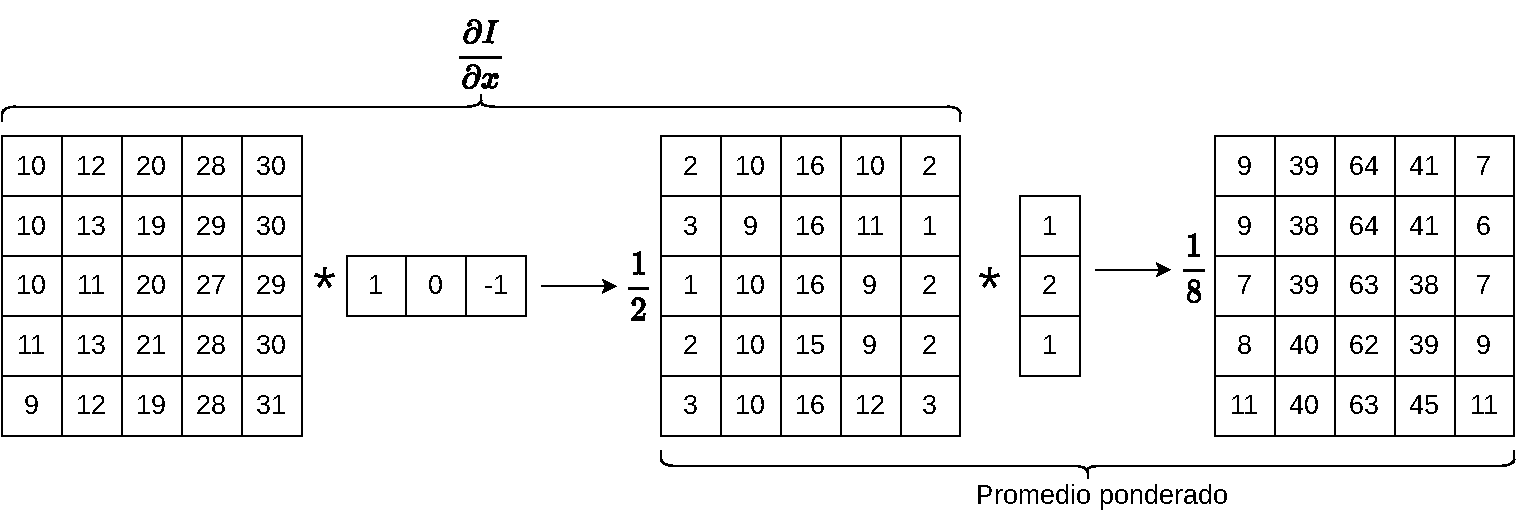
\includegraphics[width=\textwidth]{Figures/SobelX1.pdf}
  Se realiza un proceso similar para la derivada parcial en $Y$. Aplicando la propiedad asociativa de la convolución, se obtienen los siguientes ekernels:
  \[S_x = \left[\begin{tabular}{ccc}1 & 0 & -1\\2 & 0 & -2\\1 & 0 & -1 \end{tabular}\right]\qquad\qquad
  S_y = \left[\begin{tabular}{ccc}1 & 2 & 1\\0 & 0 & 0\\-1 & -2 & -1 \end{tabular}\right]\]
\end{frame}

\begin{frame}\frametitle{Ejemplo}
\end{frame}

\begin{frame}\frametitle{Magnitud y Ángulo}
  El gradiente en cada pixel de la imagen se puede calcular mediante la approximación de las derivadas parciales:
  \begin{eqnarray*}
    \frac{\partial I}{\partial x} &\approx& I * Sx = G_x\\
    \frac{\partial I}{\partial y} &\approx& I * Sy = G_y\\
  \end{eqnarray*}
  En la mayoría de las aplicaciones es más últil expresar el gradiente en forma polar:
  \[ \nabla I = G_m \angle G_a \]
  Donde la magnitud del gradiente y la fase, para cada pixel, se calculan como:
  \begin{eqnarray*}
    G_{m_{i,j}} &=& \sqrt{G_{x_{i,j}}^2 + G_{y_{i,j}}^2}\\
    G_{a_{i,j}} &=& \atantwo(G_{y_{i,j}}, G_{y_{i,j}})\\
  \end{eqnarray*}
\end{frame}

\begin{frame}\frametitle{Detector de Bordes de Canny}
  El detector de bordes de Canny es un detector basado en gradiente que consta de los siguientes pasos básicos:
  \begin{enumerate}
  \item Obtención del gradiente en magnitud y ángulo, mediante operadores de Sobel
  \item Supresión de puntos no máximos
  \item Aplicación de un doble umbral
  \end{enumerate}
  Aunque no es un paso en sí del Detector de Canny, generalmente se considera como primer paso la aplicación de un filtro Gaussiano para disminuir el ruido. 
\end{frame}

\begin{frame}\frametitle{Obtención del gradiente}
  Después del filtro Gaussiano, el primer paso es obtener el gradiente de la imagen mediante el Filtro de Sobel, en la forma de magnitud y ángulo:\\
  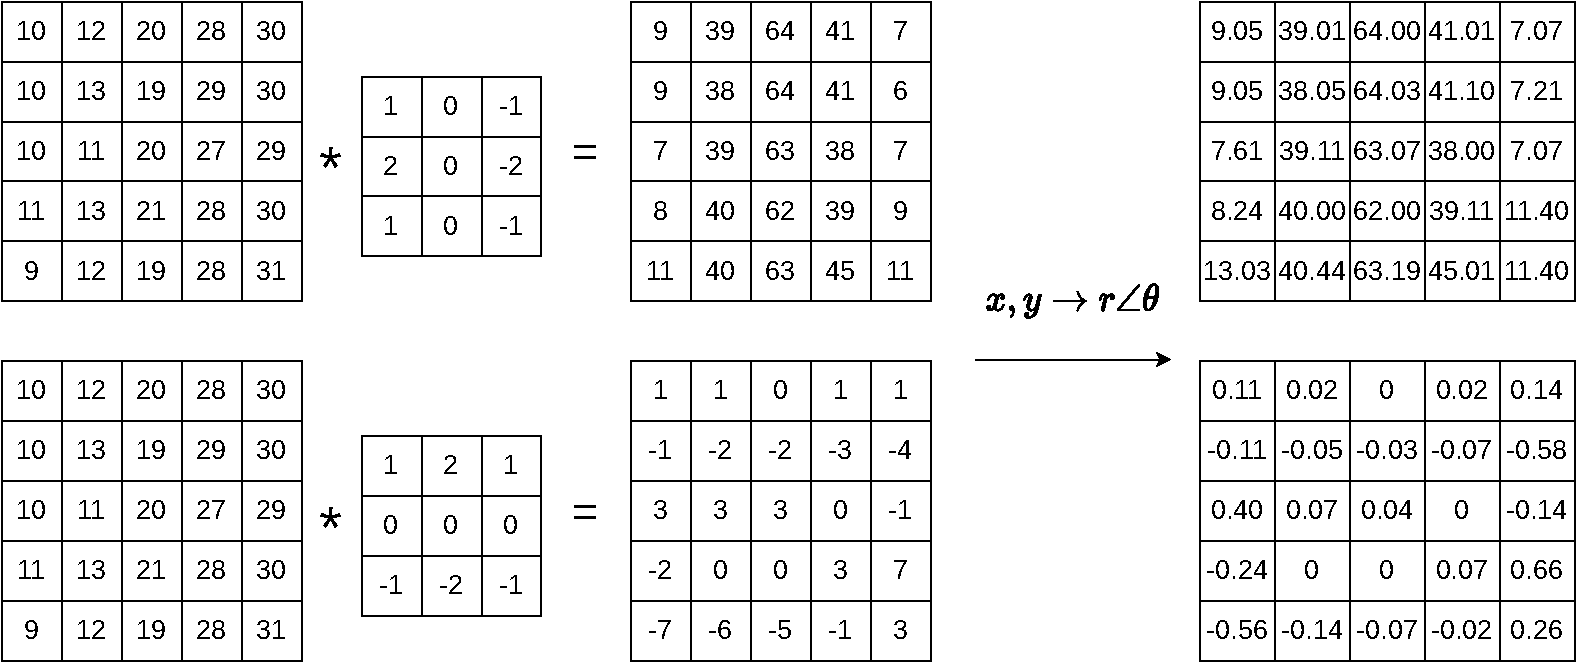
\includegraphics[width=0.9\textwidth]{Figures/SobelXY.pdf}
\end{frame}

\begin{frame}\frametitle{Supresión de no máximos}
  Este paso consiste en comparar la magnitud de cada pixel, con los pixeles anterior y posterior en la dirección del gradiente.
  Aunque la fase es un ángulo en $[-\pi, \pi]$, la dirección del gradiente se debe redondear a algún valor correspondiente a la connectividad 8: \textit{N, NE, E, SE}. Debido a que el pixel se compara en la dirección positiva y negativa del gradiente, no es necesario considerar las direcciones \textit{S, SW, W, NW}.
  \begin{figure}
    \centering
    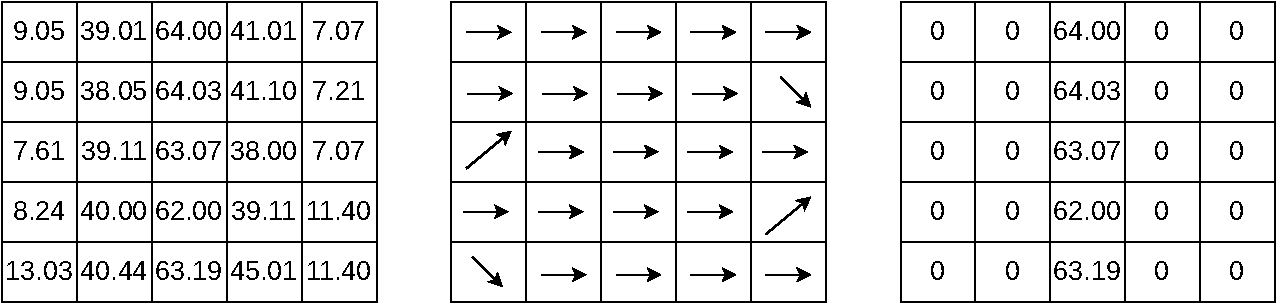
\includegraphics[width=0.9\textwidth]{Figures/SobelMA.pdf}
  \end{figure}
  Para cada pixel $p_i$, considere $p_{i+1}$, el pixel siguiente en la dirección del gradiente, y $p_{i-1}$, el pixel anterior, en la dirección del gradiente. El valor para cada pixel $q_i$ en la imagen resultante es:
  
  \[q_i = \begin{cases}p_i\qquad\qquad\textrm{si}\qquad p_i > p_{i+1} \qquad\textrm{y}\qquad p_i > p_{i-1}\\
  0\qquad\qquad\textrm{en otro caso}\end{cases}\]
\end{frame}

\begin{frame}\frametitle{Aplicación de doble umbral}
  En este paso, se definen dos umbrales: superior $\theta_u$ e inferior $\theta_l$. Los pixeles se clasifican en tres tipos:
  \begin{itemize}
  \item Fuertes: pixeles con magnitud del gradiente mayor que el umbral superior $|\nabla | > \theta_u$
  \item Débiles: pixeles con magnitud del gradiente entre ambos umbrales $\theta_l < |\nabla| < \theta_u$
  \item Suprimidos: pixeles con magnitud del gradiente menor que el umbral inferior $|\nabla| < \theta_l$
  \end{itemize}
  La imagen resultante se forma con las siguientes reglas:
  \begin{itemize}
  \item Todos los pixeles fuertes son parte de un borde.
  \item Todos los pixeles suprimidos no son bordes. 
  \item Los pixeles débiles son parte de un borde solo si están conectados (en conectividad 8) con un pixel fuerte.
  \end{itemize}
  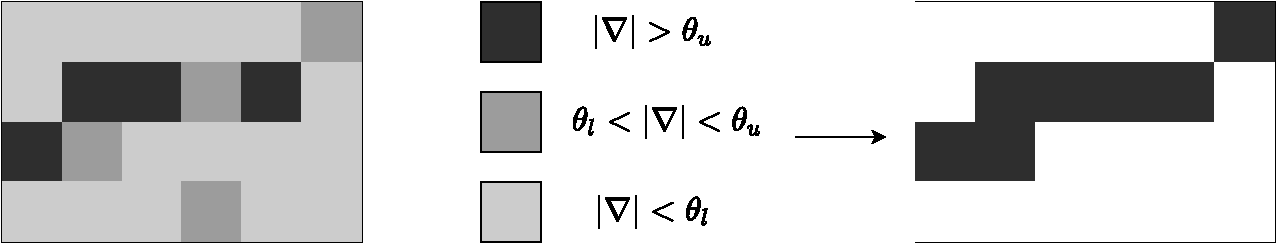
\includegraphics[width=\textwidth]{Figures/CannyDoubleThreshold.pdf}
\end{frame}

\begin{frame}\frametitle{Extracción de características}
  \begin{itemize}
  \item Las \textit{características} (\textit{features}) son conjuntos de valores derivados de una señal o de un conjunto de mediciones, que permiten describir el conjunto original y que son informativos y no redundantes.
  \item   Unas de las características más simples que se pueden extraer de una imagen son líneas y otras formas geométricas simples.
  \item El vector de características que describe una línea puede ser el conjunto de parámetros de su ecuación.
  \item Los vectores de características también se pueden utilizar para reconocer objetos, usando características cmo color, tamaño, forma, volumen, entre otras.
   \item Más adelante se verá la Transformada SIFT, uno de los algoritmos más usados para extracción de características. 
  \end{itemize}
\end{frame}

\begin{frame}\frametitle{La Transformada Hough}
  La Transformada Hough es un método que permite encontrar líneas, círculos y otras formas geométricas que se puedan describir fácilmente mediante expresiones analíticas. En el caso de las líneas, se trata de encontrar los dos parámetros que describen la recta:
  \begin{columns}
    \begin{column}{0.4\textwidth}
      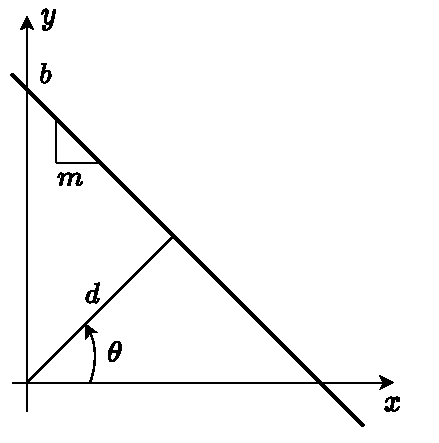
\includegraphics[width=\textwidth]{Figures/Hough2.pdf}
    \end{column}
    \begin{column}{0.6\textwidth}
      \begin{itemize}
      \item La forma pendiente-ordenada $y = mx + b$ tiene la desventaja de no poder expresar líneas verticales.
      \item La forma canónica $Ax + By + C$ requiere de una normalización $A_1 x + B_1 y + 1 = 0$ para que solo sean dos parámetros.
      \item Una forma más conveniente, es la forma normal $d = x\cos\theta + y\sin\theta$
      \item Esta última forma tiene una ventaja: si la línea correponde a un borde, el ángulo $\theta$ será la dirección del gradiente. 
      \end{itemize}
    \end{column}
  \end{columns}
\end{frame}

\begin{frame}\frametitle{El Espacio de Hough}
  El Espacio de Hough, para el caso de las líneas, es el conjunto de todos los posibles pares $(\theta, d)$.
  \begin{itemize}
  \item Una recta $L$ en el espacio cartesiano corresponde a un punto $P_h$ en el Espacio de Hough
  \item Un punto $P_c$ en el espacio cartesiano corresponde a una curva $C$ en el Espacio de Hough. Esta curva representa los parámetros $(\theta_i, d_i)$ de todas las rectas $L_i$ que pasan por el punto $P$.
  \end{itemize}
  \begin{figure}
    \centering
    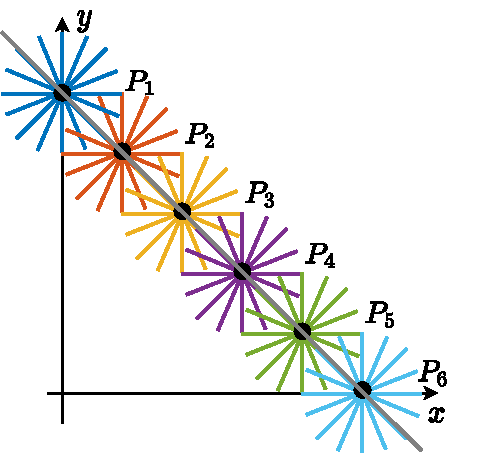
\includegraphics[width=0.35\textwidth]{Figures/Hough1.pdf}
    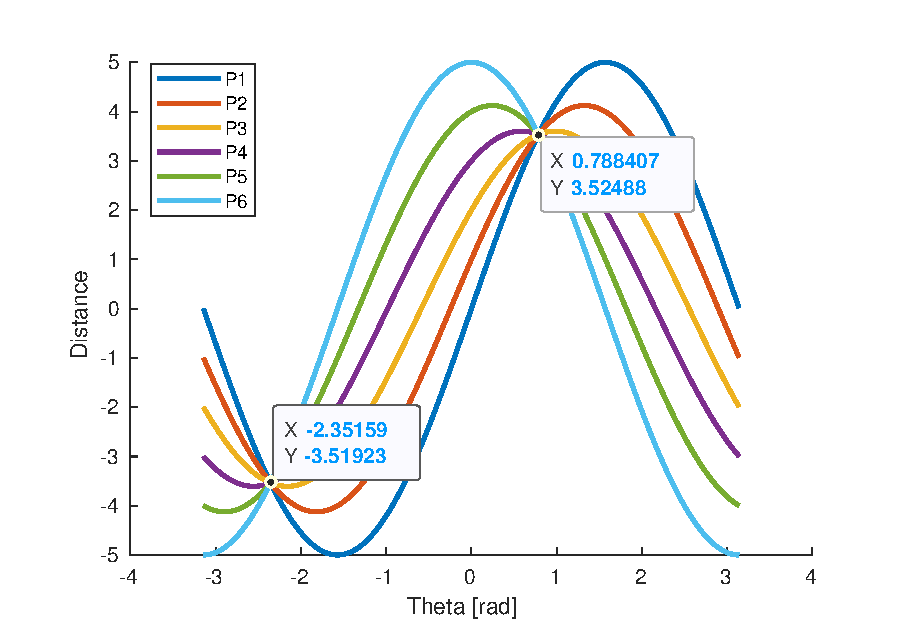
\includegraphics[width=0.5\textwidth]{Figures/Hough1.eps}
  \end{figure}
\end{frame}

\begin{frame}\frametitle{Extracción de Líneas por Transformada Hough}
  Este método consiste en encontrar las curvas $C_i$ en el espacio de Hough que pasan por cada punto $P_c$ en el espacio cartesiano. Los puntos $P_h$ en el Espacio de Hough por donde pasen más curvas $C_i$ corresponderán a las rectas resultantes en el espacio cartesiano.
  \begin{figure}
    \centering
    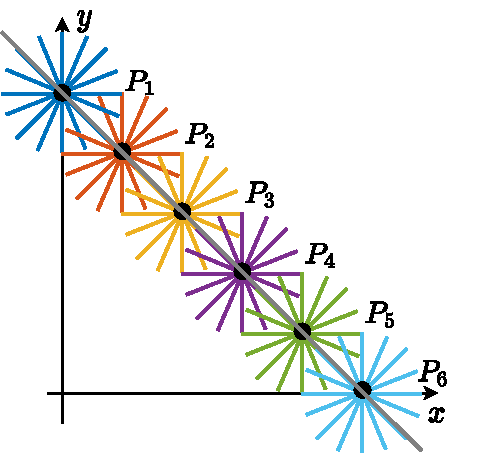
\includegraphics[width=0.35\textwidth]{Figures/Hough1.pdf}
    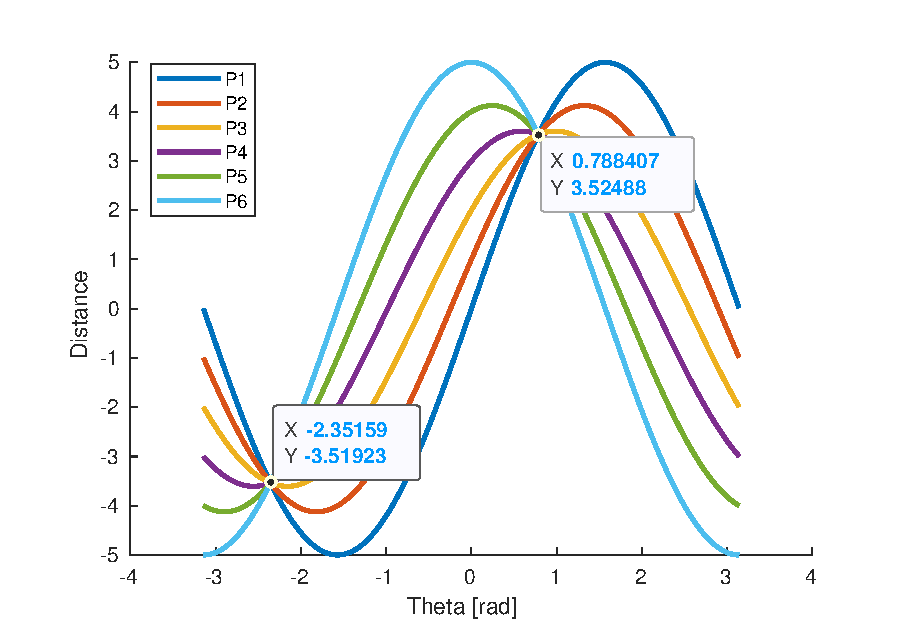
\includegraphics[width=0.5\textwidth]{Figures/Hough1.eps}
  \end{figure}
\end{frame}

\begin{frame}\frametitle{Extracción de Líneas por Transformada Hough}
  \begin{algorithm}[H]
    \KwIn{Imagen binaria $M$, umbral mínimo de votos $a_{min}$}
    \KwOut{Líneas expresadas en la forma $(d,\theta)$}
    \DontPrintSemicolon
    \;
    Inicializar en 0 un conjunto $A$ de acumuladores para cada par cuantizado $(d_k,\theta_k)$\;
    \ForAll{Pixel $M[i,j] \neq 0$}
    {
      \ForAll{Ángulo $\theta_k$ cuantizdo}
      {
        $d = j\cos\theta_k + i\sin\theta_k$
        $d_k = $ valor cuantizado de $d$
        Incrementar en uno el acumulador correspondiente $A[d_k, \theta_k]$
      }
    }
    \ForAll{$a \in A$}
    {
      \If{$a > a_{min}$}
      {
        Agregar la línea $(d_k, \theta_k)$ al conjunto de líneas detectadas
      }
    }
    Devolver el conjunto de líneas detectadas
  \end{algorithm}
\end{frame}

\begin{frame}\frametitle{Extracción de círculos por T. Hough}
  De la ecuación de un círculo en el plano:
  \[(x - c_x)^2 + (y - c_y)^2 = r^2\]
  Se puede observar que un círculo está definido por tres parámetros $(c_x, c_y, r)$.
  \begin{itemize}
  \item De forma similar a las líneas, se podrían fijar dos parámetros y calcular el tercero
  \item Sin embargo variar dos parámetros incrementa la complejidad considerablemente
  \item Se puede utilizar el ángulo del gradiente y un variar el valor del radio $r$ para determinar el centro, de este modo, solo se tiene que variar un parámetro.
  \item Se considera que el gradiente apunta hacia el centro del círculo. 
  \end{itemize}
\end{frame}

\begin{frame}\frametitle{Análisis de Componentes Principales}
  \begin{itemize}
    \item PCA representa datos en un nuevo sistema de coordenadas en que los vectores base siguen modos de mayor varianza en los datos, estas bases se
      obtienen de los datos en cuestión.
    \item PCA es un método para simplificar un conjunto de datos multidimensional a dimensiones menores para su analísis, visualización o compresión de
      datos.
      \item En la siguiente figura, si se utiliza la matriz de transformación adecuada $Q$, los puntos con respecto al nuevo sistema $X^\prime Y^\prime$ tienen componente en $Y^\prime$ muy pequeña, por lo que se podrían aproximar con una sola dimensión haciendo $Y^\prime = 0$. 
\end{itemize}
\begin{figure}
  \centering
  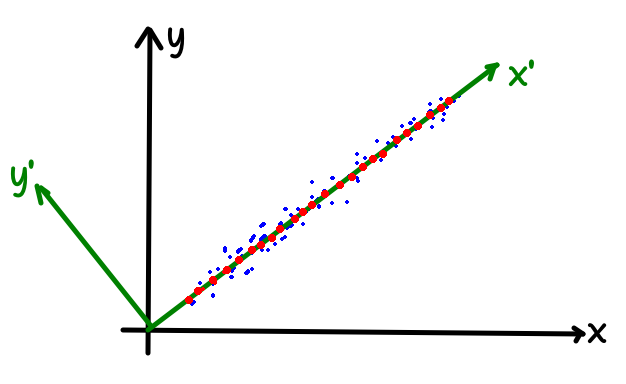
\includegraphics[width=0.4\textwidth]{Figures/PCA1.png}
\end{figure}
\end{frame}

\begin{frame}\frametitle{Análisis de componentes principales}
  \begin{columns}
    \begin{column}{0.4\textwidth}
      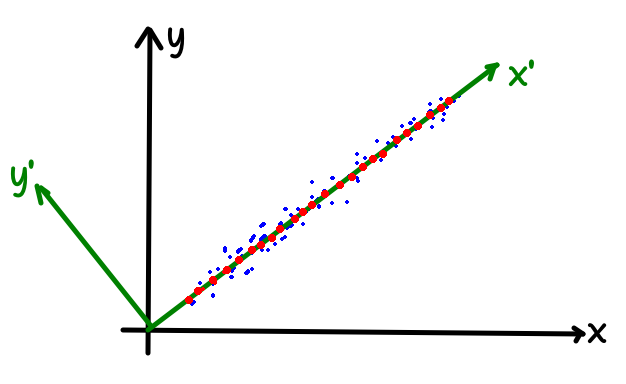
\includegraphics[width=\textwidth]{Figures/PCA1.png}
    \end{column}
    \begin{column}{0.6\textwidth}
      La matriz $Q$ se puede obtener con los siguientes pasos:
      \begin{itemize}
      \item Obtener la matriz de covarianza $P\in\mathbb{R}^{3\times 3}$ de todos los puntos
      \item Obtener los vectores propios $[v_1, v_2, v_3]$ de la matriz $P$
      \item Formar la matriz $Q$ utilizando $v$ como columnas: $Q= [v1\quad v2\quad v3]$
      \end{itemize}
    \end{column}
  \end{columns}
  Cuando se obtiene PCA para puntos en 3D puede suceder que:
  \begin{itemize}
  \item Si se tienen tres valores propios grandes, seguramente no se puede reducir la dimensión
  \item Si se tiene un valor propio pequeño y dos grandes, es probable que se tenga un plano
  \item Si se tienen dos valores propios pequeños, es probable que se trate de una recta 
  \end{itemize}
\end{frame}

\begin{frame}\frametitle{El algoritmo RANSAC}
  \begin{itemize}
  \item Sirve para ajustar los parámetros de un modelo a partir de un conjunto de observaciones cuando existen datos atípicos (\textit{outliers})
  \item Los pasos generales son los siguientes:
    \begin{enumerate}
    \item Tomar $N$ muestras aleatorias del conjunto de observaciones ($N$ suficiente para ajustar un modelo)
    \item Obtener los parámetros $\Theta$ del modelo utilizando solo esos $N$ puntos
    \item Determinar cuántos puntos del conjunto total ajustan razonablemente bien el modelo con parámetros $\Theta$
    \item Si el número de puntos que ajustaron bien supera un umbral mínimo, se acepta el modelo $\Theta$, si no, se repite el proceso 
    \end{enumerate}
  \end{itemize}
\end{frame}

\begin{frame}\frametitle{Ejercicio 09 - Características geométricas}
\end{frame}